\chapter{Conclusions}
\label{chap7}

\section{Overview}
This project looks at the problem of reconstructing shredded black and white documents, starting from a scanned image of the shreds and ending with a total or partial reconstruction of the original document. The reconstruction is split into 3 functions, ``Pre-process", ``Score" and ``Search", each of which is analysed individually. 

As part of pre-processing, we define the notion of an \emph{ideal shred} and discuss methods by which such shreds may be extracted from a real scanned image. In particular a new shred orientation method is discussed, which is computationally efficient and works well on strip-cut documents. 

The presented scoring function represents a departure from all other scoring/costs functions previously presented in literature. By adopting a probabilistic framework, we improve upon the performance of the previous state-of-the-art method while also getting rid of the ad-hoc heuristics the previous method had used to deal with issues such as white-on-white matches. Additionally, our proposed function is shown to be more robust on most noisy documents and is also more easily composed with other scoring functions, as demonstrated by its combination with ``RowScore".

We analysed the search heuristics used so far and proposed a novel ``Kruskal inspired" variant. The Kruskal heuristic outperforms the previously proposed methods and also easily lends itself to compositions with other search methods, via its ``early stopping" functionality. Finally, we analyzed a common shortcoming of the heuristics, namely a ``cascading" effect and tested out some possible solutions for this problem.

\section{Results}
\label{chap7Rez}
A major difference can be observed between the results obtained on the strip-cut and cross-cut variants, as shown in Figure\footnote{These results are obtained using virtually shredded documents, the Prim search heuristic and the probabilistic scoring function} \ref{fig:rez}.

\begin{figure}[h]
    \centering
    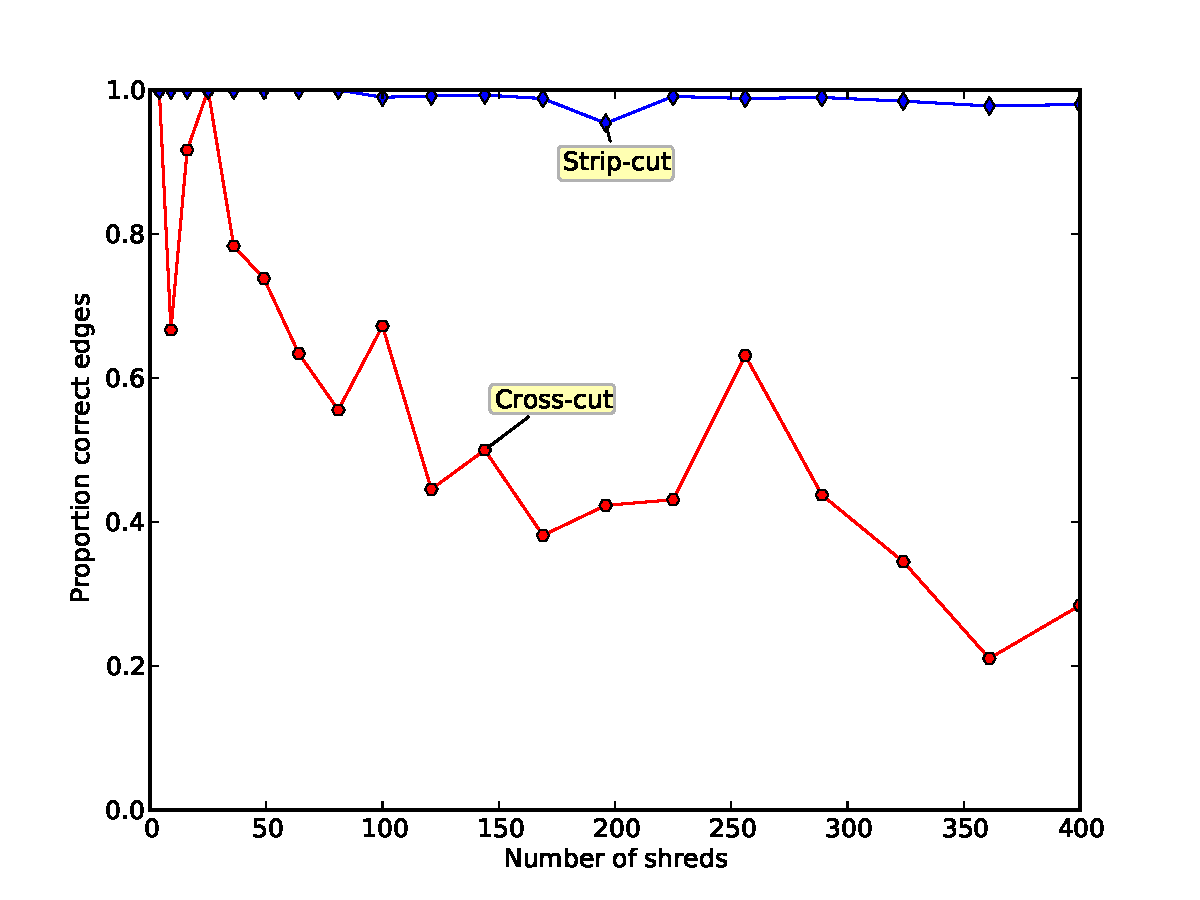
\includegraphics[width=\textwidth]{stripVsCC.pdf}
    \caption{The performance of the system on strip-cut and cross-cut documents. While the strip-cut variant is almost completely solved, the cross-cut one proves to be significantly more difficult.}
    \label{fig:rez}
\end{figure}

In order to get a better idea of what these numbers mean, we can take a look at some sample reconstructed documents. A document cut into 49 strips is shown in Figure \ref{fig:strip} and a document cross-cut into 49 rectangles is shown in Figure \ref{fig:cross}.

We can see that with a 64\% completion rate the reconstructed cross-cut document has many readable sections. Figure \ref{fig:crossGroups} shows all the subgroups of the document that were correctly reconstructed.

\begin{figure}[H]
    \centering
    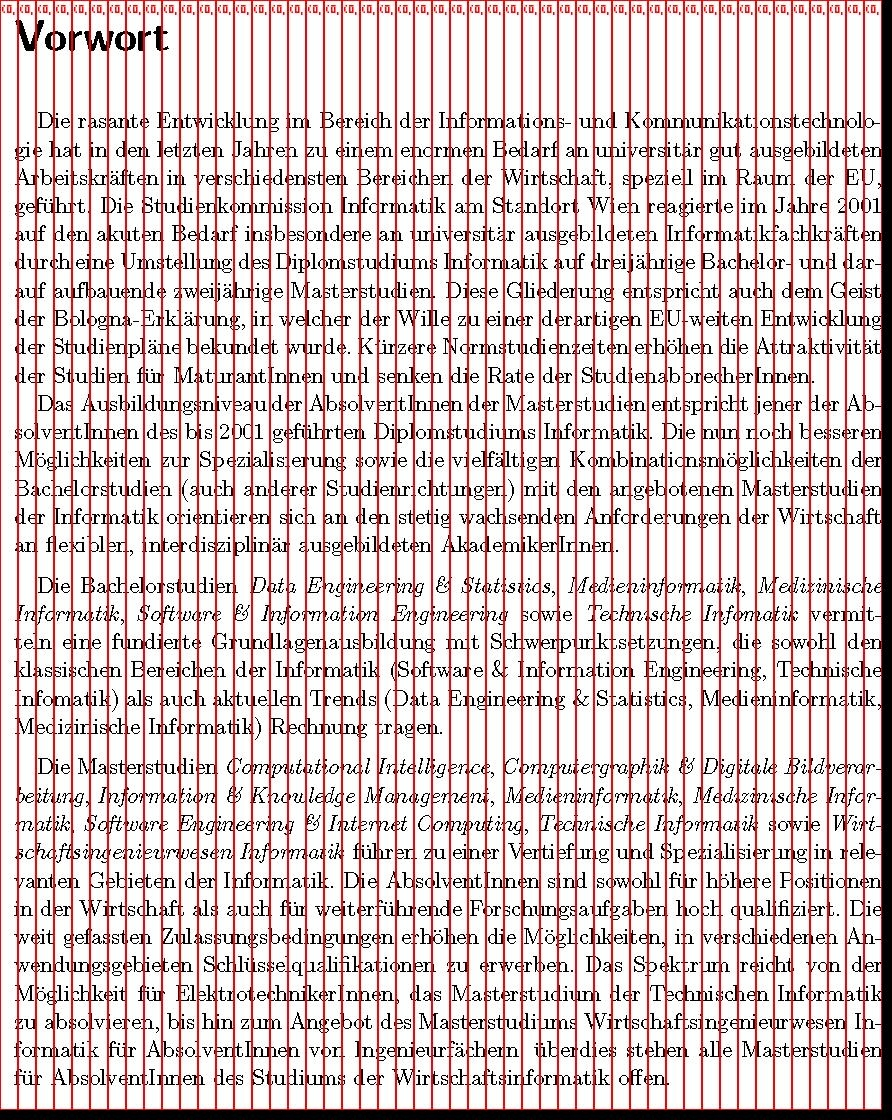
\includegraphics[width=0.9\textwidth]{prim1x49}
    \caption{As expected, the strip-cut document is perfectly reconstructed.}
    \label{fig:strip}
\end{figure}

\begin{figure}[H]
    \centering
    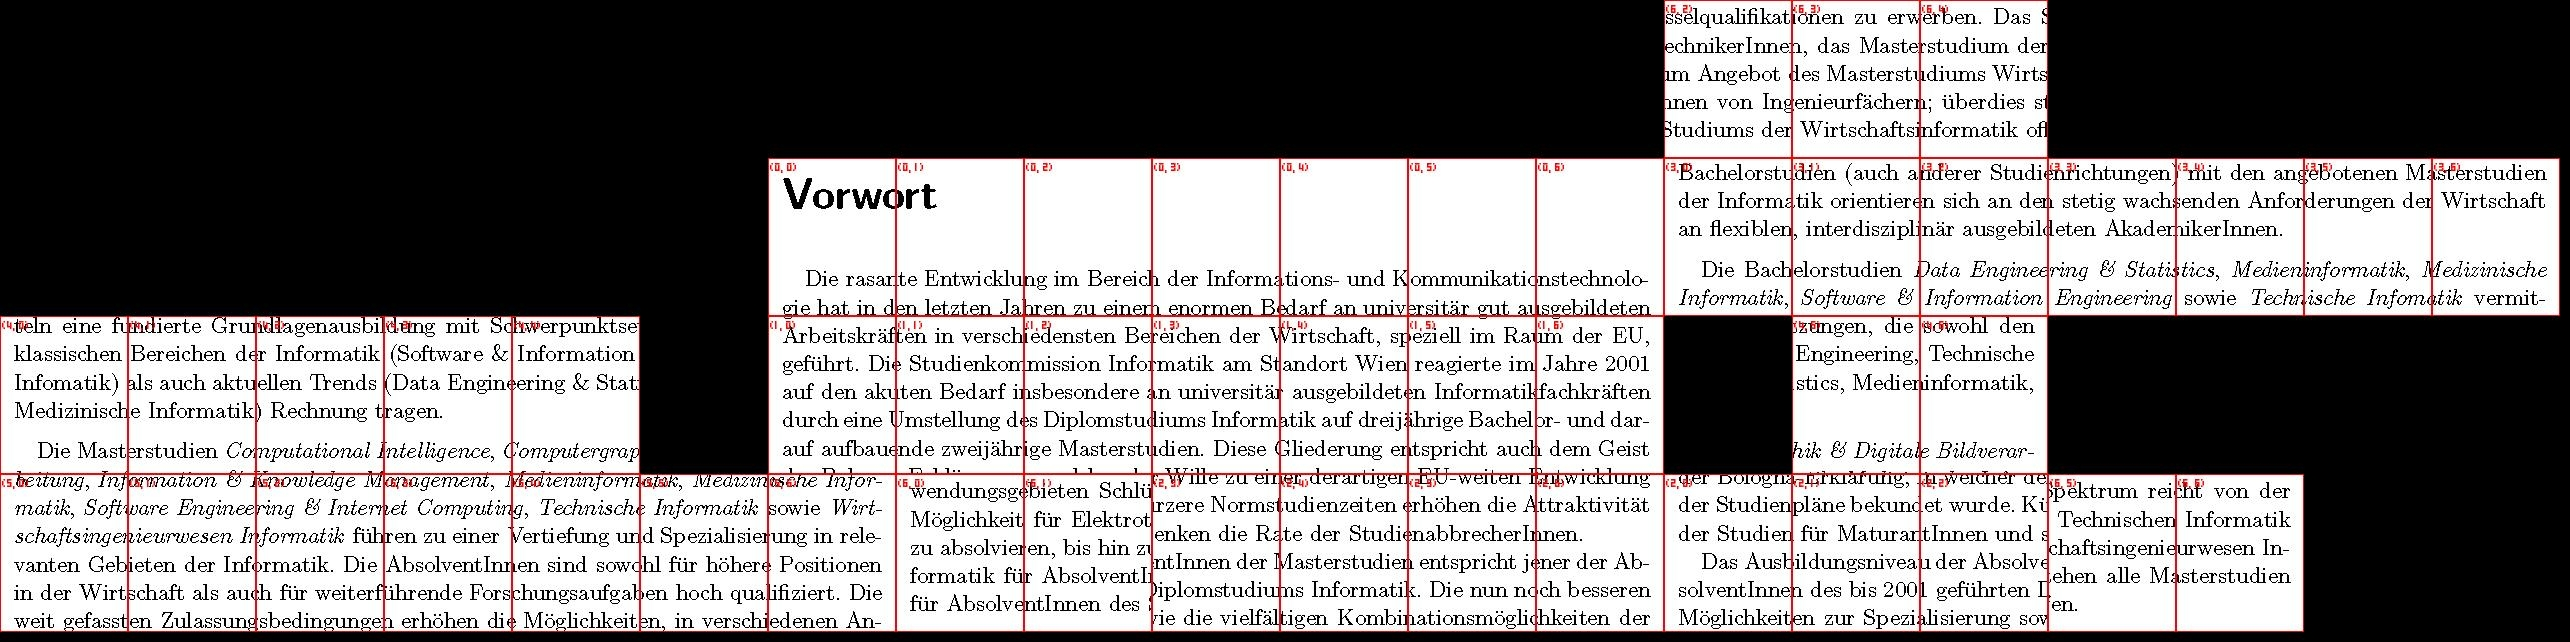
\includegraphics[width=\textwidth]{prim7x7}
    \caption{This is the outputted document for a 7x7 cross-cut. The edges in this document are 64\% correct.}
    \label{fig:cross}
\end{figure}

\begin{figure}[H]
    \centering
    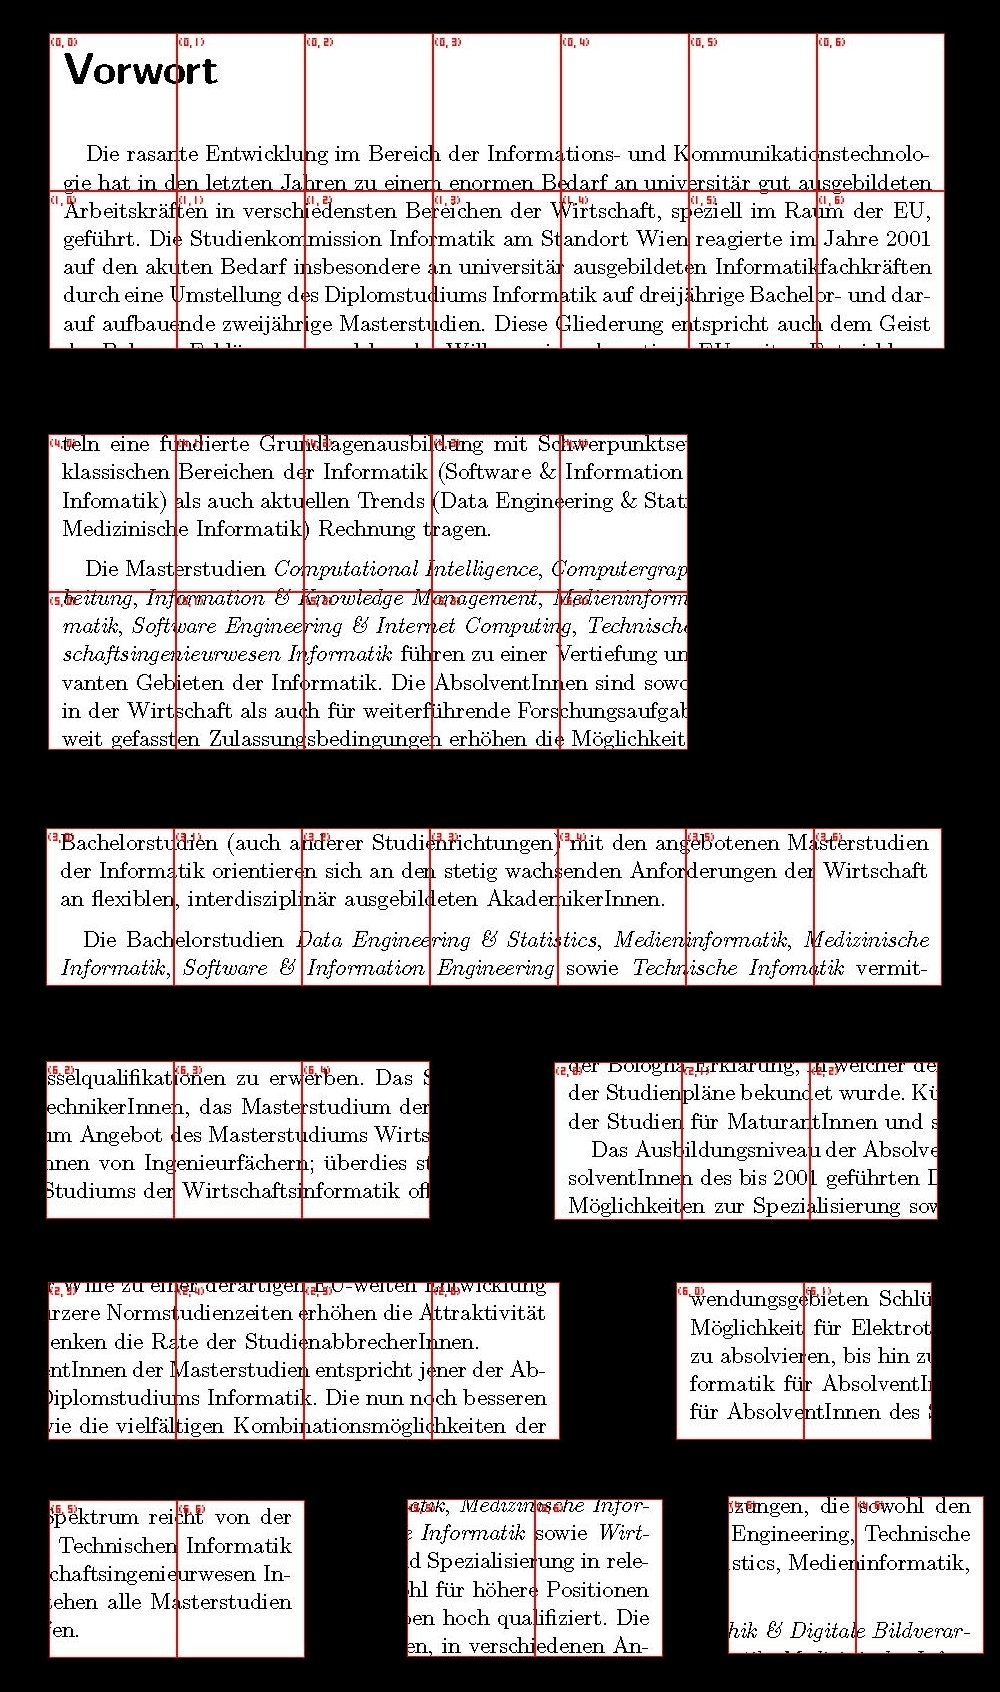
\includegraphics[width=0.8\textwidth, height=17cm]{prim7x7Groups}
    \caption{All correctly reconstructed groups of shreds from the cross-cut document. These groups were manually extracted from the reconstructed document.}
    \label{fig:crossGroups}
\end{figure}

Here, if we think in terms of the evaluation metric introduced in Section \ref{chap5Eval}, we can see that the search space has been reduced from 49 shreds to 10 shreds. Even though this only corresponds to 64\% correct edges in the final image, the reduction in search space means that, while the initial task would have been somewhat daunting to a human, the new task can be solved with relative ease. Using the ``early stopping" mechanism presented in Section \ref{chap5Mod} further simplifies the human's task by returning just the groups the algorithm is certain about. The identified groups with a threshold of 99.5\% are shown in Figure \ref{fig:stopped}.

\begin{figure}[H]
    \centering
    
\includegraphics[width=0.9\textwidth]{stopped7x7}
    \caption{The groups automatically identified by the Kruskal search with a stopping threshold of 99.5\%.}
    \label{fig:stopped}
\end{figure}

\newpage
\section{Future Work}
The post-processing step is in most dire need of work, since it isn't currently usable without spending a large amount of time and effort preparing the shreds before scanning. First of all, the problem with the ``curviness" of the strips could be managed by implementing a more complex segmentation method, such as the polynomial fitting or the Hough transform proposed in \cite{P26}. Methods of better managing the noise inherent in the shredding, scanning and processing of shreds are also necessary. If the strips are to be segmented and rotated at a high-resolution and then downsampled, the effect of different downsampling and denoising methods needs to be analysed. Lastly, more robust orientation detection methods are needed for small cross-cut documents. Some variants that could be tested include those presented in \cite{P45} and \cite{P46}.

The scoring function, at this stage, can best be improved by being composed with higher-level probabilistic scoring functions. One very simple such function, ``RowScore", was tested, but more complex variants could be incorporated. One idea would be to look at the size of the blobs of continuous black pixels formed by a new edge (i.e. the letters situated on the edge). Another method, proposed in \cite{P8} would be to look at the actual shape of the aforementioned black, continuous, blobs and predict the probability that these are real letters. Going further, new methods could be devised that do optical character recognition on the shreds and predict the likelihood of detected n-grams. Going in a different direction, different models could be proposed that expand the problem space to incorporate full-colour documents, or even hand-torn documents.

Further work on the search function should focus on fixing the cascading problem presented in Section \ref{chap5Casc}. In order to solve this problem a limited exploration of the search space likely needs to be performed. The best way to perform this exploration is an interesting problem that hasn't been previously looked at. Several other additions could also be implemented as to make the system more robust to real world conditions. For instance, the system should be able to handle double-sided documents, as well as documents that contain both text and pictures. Additionally, the degradation of the system when presented with missing shreds or with shreds that don't belong to the current document should be explored.
